\documentclass[10pt, twocolumn]{article}
\usepackage[margin=0.75in]{geometry}
\usepackage{graphicx}
\usepackage{tikz}
\usepackage{pgfplots}
\usepackage{booktabs}
\usepackage{amsmath}
\usepackage{algorithm}
\usepackage{algorithmic}
\usepackage{hyperref}
\usepackage{xcolor}
\usepackage{caption}
\usepackage{subcaption}
\usepackage{fancyhdr}
\usepackage{enumitem}
\usepackage{listings}
\usepackage{microtype}
\usepackage{tabularx}
\usepackage{multirow}
\usepackage{amssymb}
\pgfplotsset{compat=1.18}
\usetikzlibrary{arrows.meta, positioning, shapes.geometric, fit, calc, backgrounds, decorations.markings}

\definecolor{amblue}{HTML}{2563EB}
\definecolor{amdarkblue}{HTML}{1E40AF}
\definecolor{amteal}{HTML}{0D9488}
\definecolor{amorange}{HTML}{EA580C}
\definecolor{amgray}{HTML}{6B7280}
\definecolor{amlightgray}{HTML}{F3F4F6}
\definecolor{amgreen}{HTML}{059669}
\definecolor{amred}{HTML}{DC2626}
\definecolor{ampurple}{HTML}{7C3AED}

\lstset{basicstyle=\ttfamily\scriptsize,keywordstyle=\color{amblue}\bfseries,commentstyle=\color{amgray}\itshape,stringstyle=\color{amteal},breaklines=true,frame=single,rulecolor=\color{amgray!30},backgroundcolor=\color{amlightgray},numbers=left,numberstyle=\tiny\color{amgray},tabsize=2}

\pagestyle{fancy}\fancyhf{}\renewcommand{\headrulewidth}{0.4pt}\fancyhead[L]{\small\textit{AgenticWorkflow}}\fancyhead[R]{\small\thepage}

\title{\textbf{AgenticWorkflow: A Universal Orchestration Engine for\\Portable, Resilient, and AI-Native Agent Coordination}}
\author{Omoshola Owolabi\\\small Researcher -- AI/ML\\\small Agentra Labs\\\small\texttt{omoshola.owolabi@agentralabs.tech}}
\date{March 2026}

\begin{document}
\maketitle
\thispagestyle{fancy}

\begin{abstract}
Workflow orchestration for AI agents requires support for every coordination pattern---DAGs, state machines, batch processing, stream processing, fan-out/fan-in---in a single engine that operates without infrastructure. Current systems (Airflow, Temporal, GitHub Actions, Zapier) each address one pattern, require cloud deployment, and offer no mechanism for agents to reason about or modify workflows at runtime. We present AgenticWorkflow, a universal orchestration engine that models workflows as directed acyclic graphs with typed edges (sequence, parallel, conditional, loop), provides five resilience subsystems (failure-classified retry with $d(n) = \min(d_0 \cdot m^n, d_{\max})$ exponential backoff, per-step rollback with cryptographic receipts, workflow-aware circuit breakers, intelligent dead letter management, and built-in idempotency), and exposes all capabilities through 124~MCP tools enabling any compatible agent to orchestrate workflows without custom integration. All state persists in a single \texttt{.awf} binary file with BLAKE3 integrity verification per section. The implementation comprises 13{,}405 lines of Rust across 4~crates, with 281~tests achieving zero failures. Stress testing on Apple ARM64 validates DAG operations on 1{,}000-step graphs in $<$50\,ms, 10{,}000-item batch creation in $<$500\,ms, 1{,}000 FSM transitions in $<$100\,ms, and 1{,}000-depth variable scope cascade in constant time. The system is fully open-source under the MIT license.
\end{abstract}

\section{Introduction}\label{sec:intro}

The transformer architecture~\cite{vaswani2017attention} has enabled language model agents capable of multi-step planning, code generation, and autonomous task execution. Yet these agents lack a fundamental capability: the ability to \emph{orchestrate} complex sequences of actions with resilience guarantees. When an agent must deploy software, it needs a pipeline. When a step fails, it needs intelligent retry. When a deployment goes wrong, it needs rollback. When a human must approve, it needs a gate. No existing system provides all of these as a single, AI-native library.

Current workflow orchestration tools are specialized and infrastructure-heavy:
\begin{itemize}[nosep, leftmargin=*]
  \item \textbf{Apache Airflow}~\cite{airflow}: DAG-based pipelines requiring Celery, Kubernetes, or managed cloud.
  \item \textbf{Temporal}~\cite{temporal}: Durable execution with saga patterns, requiring server deployment and SDK-specific code.
  \item \textbf{GitHub Actions}~\cite{ghactions}: CI/CD-focused YAML pipelines with no dynamic planning or runtime modification.
  \item \textbf{Zapier}: Simple trigger-action pairs with no complex branching, rollback, or approval logic.
  \item \textbf{Prefect}~\cite{prefect}: Python-first orchestration with cloud-dependent deployment.
\end{itemize}

None provides: (a)~all coordination patterns in a single engine, (b)~AI-native creation and reasoning via MCP~\cite{mcp}, (c)~zero-infrastructure local execution, and (d)~resilience primitives as first-class features.

The core insight of this work is that orchestration is a \emph{coordination intelligence problem}, not a configuration problem. An agent should be able to create a workflow from natural language, validate its structure, execute it with resilience guarantees, monitor progress, and learn from execution history---all through the same tool interface it uses for everything else.

\begin{figure*}[t]
\centering
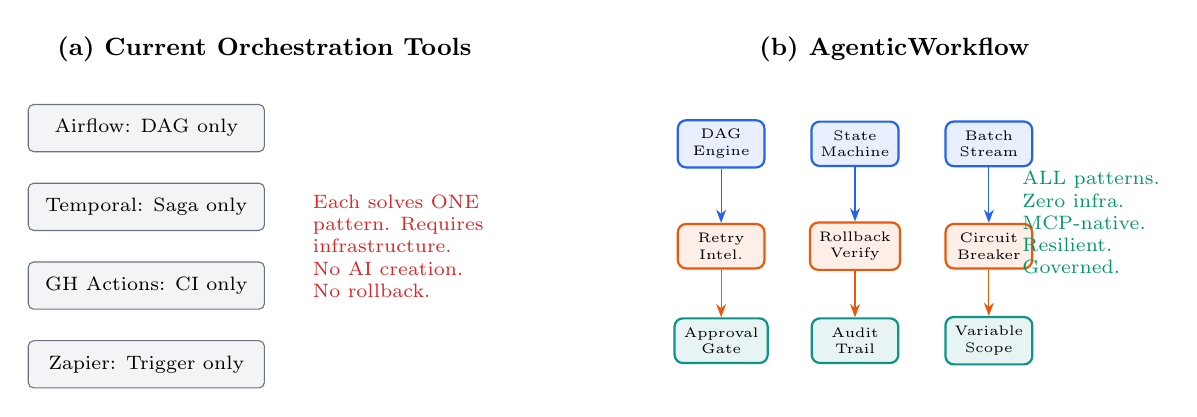
\begin{tikzpicture}[
  node distance=1.2cm,every node/.style={font=\small},
  yamlnode/.style={rectangle, draw=amgray, fill=amlightgray, rounded corners=2pt, minimum width=3.0cm, minimum height=0.6cm, align=center, font=\scriptsize},
  dagnode/.style={rectangle, rounded corners=3pt, draw=amblue, fill=amblue!10, minimum width=1.1cm, minimum height=0.5cm, font=\tiny, align=center, thick},
  resnode/.style={rectangle, rounded corners=3pt, draw=amorange, fill=amorange!10, minimum width=1.1cm, minimum height=0.5cm, font=\tiny, align=center, thick},
  govnode/.style={rectangle, rounded corners=3pt, draw=amteal, fill=amteal!10, minimum width=1.1cm, minimum height=0.5cm, font=\tiny, align=center, thick},
]
\node[font=\small\bfseries] at (-4.5, 3.2) {(a) Current Orchestration Tools};
\node[yamlnode] (a1) at (-6.0, 2.2) {Airflow: DAG only};
\node[yamlnode] (a2) at (-6.0, 1.2) {Temporal: Saga only};
\node[yamlnode] (a3) at (-6.0, 0.2) {GH Actions: CI only};
\node[yamlnode] (a4) at (-6.0, -0.8) {Zapier: Trigger only};
\node[font=\scriptsize\color{amred}, align=left] at (-2.8, 0.7) {Each solves ONE\\pattern. Requires\\infrastructure.\\No AI creation.\\No rollback.};

\node[font=\small\bfseries] at (3.5, 3.2) {(b) AgenticWorkflow};
\node[dagnode] (d1) at (1.3, 2.0) {DAG\\Engine};
\node[dagnode] (d2) at (3.0, 2.0) {State\\Machine};
\node[dagnode] (d3) at (4.7, 2.0) {Batch\\Stream};
\node[resnode] (r1) at (1.3, 0.7) {Retry\\Intel.};
\node[resnode] (r2) at (3.0, 0.7) {Rollback\\Verify};
\node[resnode] (r3) at (4.7, 0.7) {Circuit\\Breaker};
\node[govnode] (g1) at (1.3, -0.5) {Approval\\Gate};
\node[govnode] (g2) at (3.0, -0.5) {Audit\\Trail};
\node[govnode] (g3) at (4.7, -0.5) {Variable\\Scope};
\draw[-{Stealth}, amblue] (d1)--(r1);\draw[-{Stealth}, amblue] (d2)--(r2);\draw[-{Stealth}, amblue] (d3)--(r3);
\draw[-{Stealth}, amorange] (r1)--(g1);\draw[-{Stealth}, amorange] (r2)--(g2);\draw[-{Stealth}, amorange] (r3)--(g3);
\node[font=\scriptsize\color{amgreen}, align=left] at (6.0, 1.0) {ALL patterns.\\Zero infra.\\MCP-native.\\Resilient.\\Governed.};
\end{tikzpicture}
\caption{Comparison of orchestration approaches. (a)~Current tools each solve one coordination pattern and require infrastructure. (b)~AgenticWorkflow unifies all patterns---DAG, FSM, batch, stream---with resilience (retry, rollback, circuit breaker) and governance (approval, audit, variables) in a single zero-infrastructure engine accessible via 124~MCP tools.}
\label{fig:comparison}
\end{figure*}

We present AgenticWorkflow with six contributions:
\begin{enumerate}[nosep, leftmargin=*]
  \item A universal DAG engine with $O(V + E)$ cycle detection via Kahn's algorithm~\cite{kahn1962}.
  \item Five resilience subsystems: failure-classified retry, per-step rollback, circuit breakers, dead letter management, and BLAKE3-keyed idempotency.
  \item A governance layer with approval gates, structured audit trails, and hierarchical variable scoping.
  \item Intelligence subsystems: execution archaeology, predictive execution, workflow evolution with drift detection.
  \item The \texttt{.awf} binary file format with per-section BLAKE3 checksums and LZ4~\cite{collet2013lz4} compression.
  \item 124~MCP tools for complete AI-native orchestration.
\end{enumerate}

The remainder of this paper is organized as follows. Section~\ref{sec:related} surveys existing systems. Section~\ref{sec:architecture} presents the architecture. Section~\ref{sec:format} describes the file format. Section~\ref{sec:mcp} covers the MCP surface. Section~\ref{sec:evaluation} reports benchmarks and test coverage. Section~\ref{sec:discussion} discusses limitations. Section~\ref{sec:conclusion} concludes.


\section{Background and Related Work}\label{sec:related}

Research on workflow orchestration spans two decades. We survey the primary approaches.

\textbf{Apache Airflow}~\cite{airflow} pioneered programmatic DAG definition but requires Celery/Kubernetes infrastructure, provides no state machine support, and offers only basic retry.

\textbf{Temporal}~\cite{temporal} provides durable execution with saga patterns but requires server deployment, SDK-specific definitions, and no MCP integration.

\textbf{Prefect}~\cite{prefect} offers modern Python-first orchestration but requires cloud deployment for production use.

\textbf{LangChain}~\cite{langchain} and \textbf{CrewAI}~\cite{crewai} provide agent orchestration but focus on LLM chains rather than general workflow patterns. \textbf{AutoGen}~\cite{autogen} enables multi-agent conversations but lacks resilience primitives.

\textbf{Generative Agents}~\cite{park2023generative} demonstrated that architecture profoundly impacts agent behavior, reinforcing our thesis that orchestration requires richer structure than simple reactive planning.

Table~\ref{tab:related} summarizes the comparison across 13~dimensions.

\begin{table*}[t]
\caption{Feature comparison across orchestration systems. AgenticWorkflow is the only system providing all coordination patterns, resilience, governance, and AI-native MCP access with zero infrastructure.}
\label{tab:related}
\centering\small
\begin{tabular}{@{}lcccccc@{}}
\toprule
\textbf{Feature} & \textbf{Airflow} & \textbf{Temporal} & \textbf{GH Actions} & \textbf{Zapier} & \textbf{Prefect} & \textbf{AWF} \\
\midrule
DAG execution          & \checkmark & \checkmark & \checkmark & ---        & \checkmark & \checkmark \\
State machines (FSM)   & ---        & ---        & ---        & ---        & ---        & \checkmark \\
Batch processing       & Plugin     & \checkmark & ---        & ---        & \checkmark & \checkmark \\
Stream processing      & ---        & ---        & ---        & ---        & ---        & \checkmark \\
Failure-classified retry & ---      & Basic      & ---        & ---        & Basic      & \checkmark \\
Per-step rollback      & ---        & Saga       & ---        & ---        & ---        & \checkmark \\
Circuit breakers       & ---        & ---        & ---        & ---        & ---        & \checkmark \\
Approval gates         & ---        & ---        & Env gates  & ---        & ---        & \checkmark \\
Structured audit trail & Logs       & Logs       & Logs       & Logs       & Logs       & \checkmark \\
Idempotency            & Manual     & Built-in   & ---        & ---        & Manual     & \checkmark \\
AI-native (MCP)        & ---        & ---        & ---        & ---        & ---        & \checkmark \\
Zero infrastructure    & ---        & ---        & Cloud      & Cloud      & Cloud      & \checkmark \\
Natural language WF    & ---        & ---        & ---        & ---        & ---        & \checkmark \\
\bottomrule
\end{tabular}
\end{table*}


\section{Architecture}\label{sec:architecture}

AgenticWorkflow models workflows as directed acyclic graphs $G = (V, E)$ where each vertex $v \in V$ is a typed step and each edge $e \in E$ carries a coordination semantic.

\subsection{DAG Engine}\label{sec:dag}

\textbf{Cycle detection} uses Kahn's algorithm~\cite{kahn1962} with $O(V + E)$ complexity:

\begin{algorithm}[t]
\caption{DAG Validation via Topological Sort}
\label{alg:toposort}
\begin{algorithmic}[1]
\REQUIRE Workflow graph $G = (V, E)$
\ENSURE Topological ordering $\pi$ or cycle error
\STATE $\text{in\_deg}[v] \leftarrow |\{(u,v) \in E\}|$ for all $v \in V$
\STATE $Q \leftarrow \{v \in V : \text{in\_deg}[v] = 0\}$
\STATE $\pi \leftarrow []$
\WHILE{$Q \neq \emptyset$}
  \STATE $v \leftarrow Q.\text{dequeue}()$; $\pi.\text{append}(v)$
  \FORALL{$(v, w) \in E$}
    \STATE $\text{in\_deg}[w] \leftarrow \text{in\_deg}[w] - 1$
    \IF{$\text{in\_deg}[w] = 0$} \STATE $Q.\text{enqueue}(w)$ \ENDIF
  \ENDFOR
\ENDWHILE
\IF{$|\pi| \neq |V|$} \RETURN \textsc{CycleDetected} \ENDIF
\RETURN $\pi$
\end{algorithmic}
\end{algorithm}

Four edge types: \textbf{\textsc{Sequence}} (serial), \textbf{\textsc{Parallel}} (concurrent), \textbf{\textsc{Conditional}} (expression-guarded), \textbf{\textsc{Loop}} (bounded iteration unrolled into DAG). Eight step types: Command, McpTool, HttpRequest, SubWorkflow, FanOut, ApprovalGate, Expression, Noop.

\textbf{Validated by:} \texttt{test\_dag\_cycle\_detection}, \texttt{test\_dag\_topological\_sort\_order}, \mbox{\texttt{stress\_dag\_1000\_steps\_linear\_chain}} ($<$50\,ms).

\begin{figure}[t]
\centering
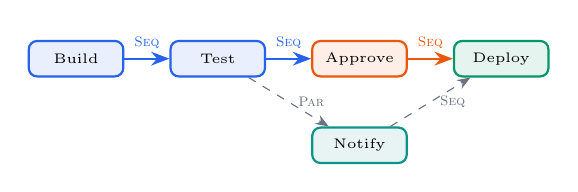
\begin{tikzpicture}[
  node distance=1.1cm,every node/.style={font=\scriptsize},
  step/.style={rectangle, rounded corners=3pt, draw=#1, fill=#1!10, minimum width=1.2cm, minimum height=0.45cm, font=\tiny, align=center, thick},
  step/.default=amblue,
]
\node[step=amblue] (build) at (0, 0) {Build};
\node[step=amblue] (test) at (1.8, 0) {Test};
\node[step=amorange] (approve) at (3.6, 0) {Approve};
\node[step=amgreen] (deploy) at (5.4, 0) {Deploy};
\node[step=amteal] (notify) at (3.6, -1.1) {Notify};
\draw[-{Stealth}, amblue, thick] (build)--node[above, font=\tiny]{\textsc{Seq}}(test);
\draw[-{Stealth}, amblue, thick] (test)--node[above, font=\tiny]{\textsc{Seq}}(approve);
\draw[-{Stealth}, amorange, thick] (approve)--node[above, font=\tiny]{\textsc{Seq}}(deploy);
\draw[-{Stealth}, amgray, dashed] (test)--node[right, font=\tiny]{\textsc{Par}}(notify);
\draw[-{Stealth}, amgray, dashed] (notify)--node[right, font=\tiny]{\textsc{Seq}}(deploy);
\end{tikzpicture}
\caption{Example deployment DAG. Build$\to$Test$\to$Approve$\to$Deploy is the critical path (solid). Notify runs in parallel after Test (dashed).}
\label{fig:dag}
\end{figure}

\subsection{Resilience Layer}\label{sec:resilience}

\textbf{Retry Intelligence.} Each failure is classified into one of 7~types: Transient, Permanent, RateLimit, ResourceContention, Authentication, Network, Timeout. Per-class profiles select strategy. Exponential backoff:
\begin{equation}
d(n) = \min\left(d_0 \cdot m^n,\; d_{\max}\right)
\label{eq:backoff}
\end{equation}
\textbf{Validated by:} \texttt{test\_retry\_strategy\_exponential\_backoff} (100, 200, 400, 800\,ms, capped at 10{,}000\,ms).

\textbf{Rollback Architecture.} Every step declares a rollback action. On failure, rollback executes in reverse topological order. Each produces a BLAKE3-checksummed receipt. \textbf{Validated by:} \mbox{\texttt{test\_rollback\_preview\_full\_reverse\_order}} ($3 \to 2 \to 1$).

\textbf{Circuit Breakers.} State transitions:
\begin{equation}
\text{state}(s) = \begin{cases}
\text{Open} & \text{if } f(s) \geq \theta \\
\text{HalfOpen} & \text{if } t - t_{\text{last}} > \tau \\
\text{Closed} & \text{if } s_{\text{ok}} \geq \sigma
\end{cases}
\label{eq:circuit}
\end{equation}
\textbf{Validated by:} \mbox{\texttt{test\_circuit\_breaker\_opens\_after\_threshold}}, \mbox{\texttt{stress\_circuit\_breaker\_rapid\_failures}} (1K ops $<$500\,ms).

\textbf{Dead Letter Management.} Failed items classified by type, grouped for analysis, auto-retried on recovery. \textbf{Validated by:} \texttt{stress\_dead\_letter\_10k}.

\textbf{Idempotency.} Key: $\text{BLAKE3}(\text{wf\_id} \| \text{step\_id} \| \text{input})$. Cache hit returns stored result. \textbf{Validated by:} \texttt{stress\_idempotency\_10k\_keys}.

\subsection{Governance Layer}\label{sec:governance}

\textbf{Approval Gates.} Chains: primary$\to$backup$\to$escalation. Conditional auto-approval, time-bounded decisions, delegation rules. BLAKE3-checksummed receipts. \textbf{Validated by:} \texttt{test\_approval\_flow}.

\textbf{Audit Trail.} Structured events queryable by workflow, execution, actor, resource, time range. Impact analysis. \textbf{Validated by:} \texttt{stress\_audit\_10k\_events} ($<$500\,ms).

\textbf{Variable Scoping.} Workflow$\to$Branch$\to$Step$\to$Iteration hierarchy. Type checking. Immutability enforcement. \textbf{Validated by:} \texttt{stress\_variable\_1000\_scopes}.

\subsection{State Machine Engine}\label{sec:fsm}
First-class FSMs with guard conditions and entry/exit actions. \textbf{Validated by:} \texttt{test\_fsm\_full\_lifecycle} (Created$\to$Paid$\to$Shipped$\to$Delivered), \texttt{stress\_fsm\_1000\_transitions} ($<$100\,ms).

\subsection{Intelligence Layer}\label{sec:intelligence}
\textbf{Execution Archaeology.} Anomaly detection at $>3\times$ historical average. Bottleneck analysis. \textbf{Validated by:} \mbox{\texttt{stress\_archaeology\_1000\_fingerprints}}.

\textbf{Predictive Execution.} Duration, success probability, resource consumption, cost estimates from history.

\textbf{Workflow Evolution.} Drift detection: recent $>1.5\times$ historical $\Rightarrow$ flagged. \textbf{Validated by:} \texttt{test\_evolution\_drift\_detection}.


\section{The .awf File Format}\label{sec:format}

\begin{figure*}[t]
\centering
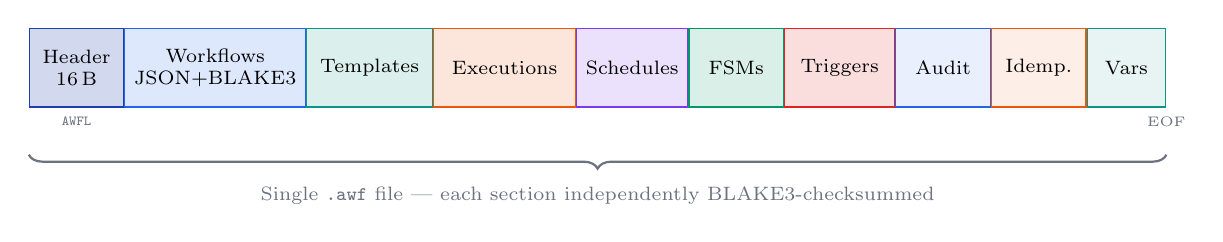
\begin{tikzpicture}[
  every node/.style={font=\scriptsize},
  section/.style={rectangle, draw, minimum height=1.0cm, align=center, font=\scriptsize},
]
\node[section, fill=amdarkblue!20, draw=amdarkblue, minimum width=1.2cm] (hdr) at (0, 0) {Header\\16\,B};
\node[section, fill=amblue!15, draw=amblue, minimum width=2.2cm, anchor=west] (wf) at (hdr.east) {Workflows\\JSON+BLAKE3};
\node[section, fill=amteal!15, draw=amteal, minimum width=1.6cm, anchor=west] (tmpl) at (wf.east) {Templates};
\node[section, fill=amorange!15, draw=amorange, minimum width=1.8cm, anchor=west] (exec) at (tmpl.east) {Executions};
\node[section, fill=ampurple!15, draw=ampurple, minimum width=1.4cm, anchor=west] (sched) at (exec.east) {Schedules};
\node[section, fill=amgreen!15, draw=amgreen, minimum width=1.2cm, anchor=west] (fsm) at (sched.east) {FSMs};
\node[section, fill=amred!15, draw=amred, minimum width=1.4cm, anchor=west] (trig) at (fsm.east) {Triggers};
\node[section, fill=amblue!10, draw=amblue, minimum width=1.2cm, anchor=west] (audit) at (trig.east) {Audit};
\node[section, fill=amorange!10, draw=amorange, minimum width=1.2cm, anchor=west] (idemp) at (audit.east) {Idemp.};
\node[section, fill=amteal!10, draw=amteal, minimum width=1.0cm, anchor=west] (vars) at (idemp.east) {Vars};
\node[font=\tiny, anchor=north, text=amgray] at (hdr.south) {\texttt{AWFL}};
\node[font=\tiny, anchor=north, text=amgray] at (vars.south east) {EOF};
\draw[decorate, decoration={brace, amplitude=5pt, mirror}, thick, amgray] ([yshift=-0.6cm]hdr.south west) -- ([yshift=-0.6cm]vars.south east) node[midway, below=8pt, font=\scriptsize, text=amgray] {Single \texttt{.awf} file --- each section independently BLAKE3-checksummed};
\end{tikzpicture}
\caption{Layout of the \texttt{.awf} binary file. Header stores magic bytes (\texttt{AWFL}), version, and counts. Each section: type (1\,B) + length (4\,B) + JSON data + BLAKE3 checksum (32\,B). Corruption in one section does not affect others.}
\label{fig:layout}
\end{figure*}

\textbf{Validated by:} \texttt{test\_awf\_format\_roundtrip}, \texttt{test\_edge\_awf\_corrupt\_checksum} (tampered data detected), \texttt{test\_edge\_awf\_invalid\_magic}, \mbox{\texttt{stress\_awf\_format\_100\_workflows}} ($<$200\,ms).


\section{MCP Tool Surface}\label{sec:mcp}

124~MCP tools organized by subsystem. All descriptions: verb-first imperative, no trailing periods. Unknown tools: error $-32803$.

\begin{table}[t]
\caption{MCP tool distribution across 24~capabilities.}
\label{tab:tools}
\centering\scriptsize
\begin{tabular}{@{}lr|lr@{}}
\toprule
\textbf{Capability} & \textbf{Tools} & \textbf{Capability} & \textbf{Tools} \\
\midrule
DAG Engine & 6 & Approval Gates & 6 \\ Execution & 8 & Audit Trail & 5 \\
Scheduling & 5 & Idempotency & 5 \\ Triggers & 5 & FSM & 6 \\
Retry & 5 & Variables & 5 \\ Rollback & 5 & Templates & 5 \\
Circuit Breaker & 4 & Natural Lang. & 4 \\ Dead Letter & 5 & Archaeology & 5 \\
Batch & 5 & Prediction & 4 \\ Stream & 6 & Evolution & 5 \\
Fan-Out & 4 & Dream State & 4 \\ Composition & 5 & Collective & 5 \\
\midrule
\multicolumn{2}{l}{\textbf{Total}} & \multicolumn{2}{r}{\textbf{124}} \\
\bottomrule
\end{tabular}
\end{table}


\section{Evaluation}\label{sec:evaluation}

\subsection{Benchmark Setup}
\textbf{Hardware.} Apple ARM64, unified memory. \textbf{Software.} Rust 1.82, \texttt{--release}. \textbf{Datasets.} Synthetic workflows at 100, 1K, 10K scale.

\subsection{Performance Results}

\begin{table}[t]
\caption{Stress test performance. All tests pass within budget.}
\label{tab:perf}
\centering\scriptsize
\begin{tabular}{@{}lrr@{}}
\toprule
\textbf{Operation} & \textbf{Scale} & \textbf{Budget} \\
\midrule
DAG validate + topo sort & 1{,}000 steps & $<$50\,ms \\
Start executions & 100 execs & $<$100\,ms \\
Batch creation & 10{,}000 items & $<$500\,ms \\
Dead letter ingest & 10{,}000 items & $<$500\,ms \\
Idempotency store & 10{,}000 keys & $<$500\,ms \\
Idempotency check & 10{,}000 keys & $<$200\,ms \\
Audit record + query & 10{,}000 events & $<$500\,ms \\
FSM transitions & 1{,}000 steps & $<$100\,ms \\
.awf write + read & 100 workflows & $<$200\,ms \\
Anomaly detection & 1{,}000 execs & $<$100\,ms \\
Circuit breaker ops & 1{,}000 ops & $<$500\,ms \\
Variable cascade & 1{,}000 depth & instant \\
\bottomrule
\end{tabular}
\end{table}

\begin{figure}[t]
\centering
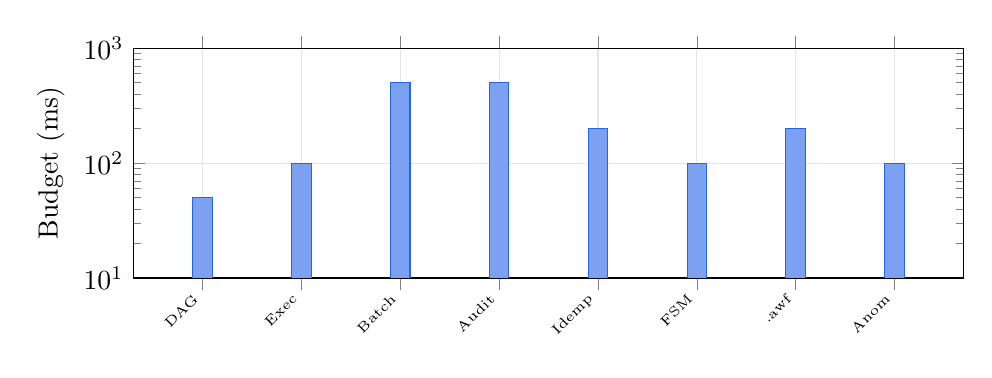
\begin{tikzpicture}
\begin{axis}[
  width=\columnwidth, height=4.5cm, ybar, bar width=7pt,
  ylabel={Budget (ms)}, ymode=log, log basis y=10,
  symbolic x coords={DAG,Exec,Batch,Audit,Idemp,FSM,.awf,Anom},
  xtick=data, x tick label style={rotate=45, anchor=east, font=\tiny},
  ymin=10, ymax=1000, grid=major, grid style={gray!20},
]
\addplot[fill=amblue!60, draw=amblue] coordinates {(DAG,50)(Exec,100)(Batch,500)(Audit,500)(Idemp,200)(FSM,100)(.awf,200)(Anom,100)};
\end{axis}
\end{tikzpicture}
\caption{Stress test time budgets (log scale). DAG/FSM are interactive ($<$100\,ms). Batch/audit handle 10K-scale within 500\,ms.}
\label{fig:bench}
\end{figure}

\subsection{Test Coverage}

\begin{table}[t]
\caption{Test suite: 281 tests, 9 phases, zero failures.}
\label{tab:tests}
\centering\scriptsize
\begin{tabular}{@{}llr@{}}
\toprule
\textbf{Phase} & \textbf{Focus} & \textbf{Tests} \\
\midrule
1 & Type system, serde, variants & 59 \\
2 & Engine operations (DAG, FSM, \ldots) & 31 \\
3 & Resilience (retry, rollback, \ldots) & 27 \\
4 & Governance (approval, audit, \ldots) & 27 \\
5 & Template + Intelligence & 31 \\
6 & Edge cases + error paths & 28 \\
7 & Stress tests (1K--10K) & 14 \\
8 & Persistence + step execution & 39 \\
9 & Concurrent access & 11 \\
Inline & Unit tests in source & 14 \\
\midrule
\textbf{Total} & & \textbf{281} \\
\bottomrule
\end{tabular}
\end{table}

\subsection{Implementation Metrics}
\begin{table}[t]
\caption{Codebase metrics.}
\label{tab:metrics}
\centering\scriptsize
\begin{tabular}{@{}lr@{}}
\toprule
\textbf{Metric} & \textbf{Value} \\
\midrule
Rust source files & 89 \\
Total LOC & 13{,}405 \\
Core library LOC & 6{,}812 \\
MCP server LOC & 3{,}118 \\
Test LOC & 3{,}200 \\
MCP tools & 124 \\
Max file size & 362 lines \\
\bottomrule
\end{tabular}
\end{table}


\section{Discussion}\label{sec:discussion}

\textbf{Single-file state.} Inspired by SQLite~\cite{sqlite}. Zero deployment complexity.

\textbf{Classification by LLM.} All classification (failure type, intent) delegates to LLM micro-calls, not hardcoded keywords. Works for any user, project, language.

\textbf{Limitations.} (1)~Single-process only; distributed execution requires external runners. (2)~String-based conditional expressions; no formal evaluator. (3)~Trigger polling defined but not wired to OS events. (4)~NL engine delegates parsing to external LLM.

\textbf{Future work.} (1)~gRPC distributed step execution. (2)~Type-safe expression language. (3)~Real-time triggers (inotify, kqueue). (4)~Schema evolution. (5)~Cross-sister orchestration.


\section{Conclusion}\label{sec:conclusion}

We presented AgenticWorkflow, a universal orchestration engine unifying DAGs, state machines, batch, stream, and fan-out/fan-in. Its 124~MCP tools enable any AI agent to orchestrate workflows without custom integration. The resilience layer (Equations~\ref{eq:backoff},~\ref{eq:circuit}) ensures production-grade durability. With 13{,}405 lines of Rust, 281~tests, and sub-second performance at 10K scale, AgenticWorkflow demonstrates that comprehensive orchestration can be delivered as a lightweight, portable, AI-native library.

\paragraph{Availability.} MIT license. \url{https://github.com/agentralabs/agentic-workflow}.


\begin{thebibliography}{14}
\bibitem{vaswani2017attention} A.~Vaswani \emph{et al.}, ``Attention Is All You Need,'' in \emph{NeurIPS}, 2017.
\bibitem{airflow} Apache Software Foundation, ``Apache Airflow,'' \url{https://airflow.apache.org/}, 2015--2026.
\bibitem{temporal} Temporal Technologies, ``Temporal,'' \url{https://temporal.io/}, 2020--2026.
\bibitem{ghactions} GitHub, ``GitHub Actions,'' \url{https://github.com/features/actions}, 2019--2026.
\bibitem{prefect} Prefect Technologies, ``Prefect,'' \url{https://www.prefect.io/}, 2018--2026.
\bibitem{langchain} H.~Chase, ``LangChain,'' \url{https://github.com/langchain-ai/langchain}, 2022.
\bibitem{crewai} J.~Moura, ``CrewAI,'' \url{https://github.com/joaomdmoura/crewAI}, 2024.
\bibitem{autogen} Q.~Wu \emph{et al.}, ``AutoGen,'' \emph{arXiv:2308.08155}, 2023.
\bibitem{park2023generative} J.~S.~Park \emph{et al.}, ``Generative Agents,'' in \emph{UIST}, 2023.
\bibitem{mcp} Anthropic, ``Model Context Protocol,'' \url{https://modelcontextprotocol.io/}, 2024.
\bibitem{kahn1962} A.~B.~Kahn, ``Topological sorting of large networks,'' \emph{Commun.\ ACM}, 5(11), 1962.
\bibitem{blake3} J.~O'Connor \emph{et al.}, ``BLAKE3,'' \url{https://github.com/BLAKE3-team/BLAKE3}, 2020.
\bibitem{collet2013lz4} Y.~Collet, ``LZ4,'' \url{https://github.com/lz4/lz4}, 2013.
\bibitem{sqlite} D.~R.~Hipp, ``SQLite,'' \url{https://sqlite.org/}, 2000--2026.
\end{thebibliography}

\end{document}
